\documentclass[aspectratio=169,10pt]{beamer}

\usepackage[utf8]{inputenc}
\usepackage{amsmath}
\usepackage{amssymb}
\usepackage{booktabs}
\usepackage{graphicx}
\usepackage{array}
\usepackage{xcolor}

\graphicspath{{../../results/figures/paper/}{../../results/figures/exploratory/}}

\definecolor{AskBlue}{RGB}{23,63,95}
\definecolor{AskGold}{RGB}{214,137,16}
\definecolor{AskRed}{RGB}{192,57,43}

\usetheme{Madrid}
\usecolortheme{default}
\setbeamertemplate{navigation symbols}{}
\setbeamertemplate{footline}[frame number]

\setbeamercolor{title}{fg=white,bg=AskBlue}
\setbeamercolor{frametitle}{fg=white,bg=AskBlue}
\setbeamercolor{structure}{fg=AskBlue}
\setbeamercolor{block title}{fg=white,bg=AskBlue}
\setbeamercolor{block body}{fg=black,bg=black!4}
\setbeamercolor{alerted text}{fg=AskGold}

\setbeamerfont{title}{series=\bfseries,size=\large}
\setbeamerfont{frametitle}{series=\bfseries,size=\large}

\title[When More Observation Hurts]{When More Observation Hurts:\\Redundancy and Robust Clarification in Ask-or-Act}
\subtitle{CS6208 Final Presentation \quad\textbar\quad 5-min talk}
\author[Zhu Yufan]{\texorpdfstring{Zhu Yufan \\ \small A0238993J}{Zhu Yufan (A0238993J)}}
\date{April 2026}

\begin{document}

% =============================================================
\begin{frame}[plain]
  \titlepage
\end{frame}

% =============================================================
\begin{frame}{The Setup}
  \begin{columns}[T,onlytextwidth]
    \column{0.52\textwidth}
      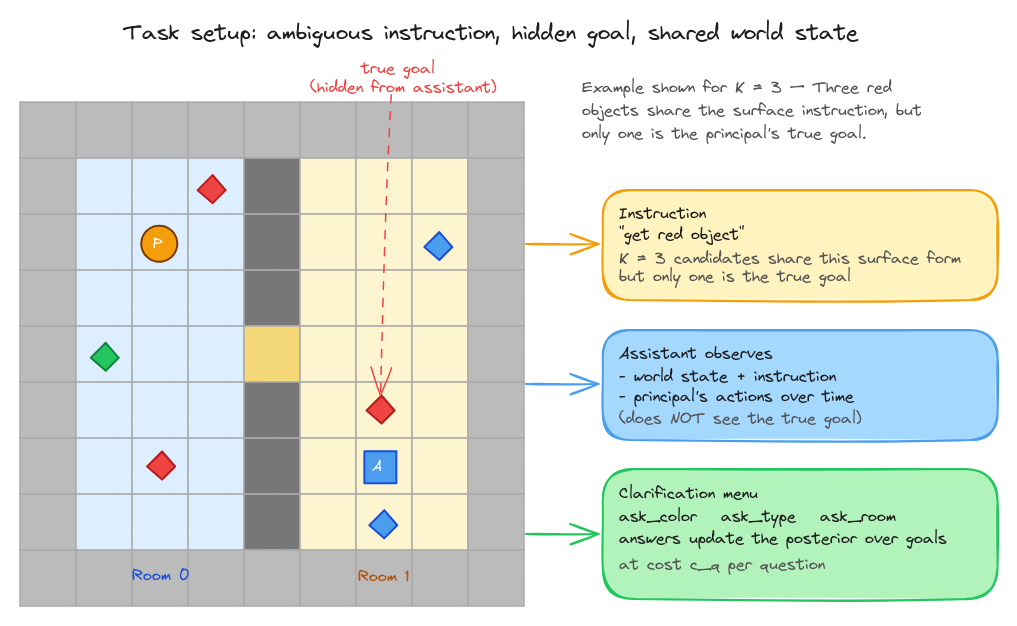
\includegraphics[width=\textwidth]{setup_overview.png}
    \column{0.46\textwidth}
      \vspace{0.6em}
      \begin{block}{Two ways to figure out a goal}
        \small
        \textbf{Watch} what the principal does, or\\
        \textbf{ask} --- at a small cost.
      \end{block}
      \vspace{0.3em}
      \begin{block}{Three policies}
        \small
        \textbf{NeverAsk} --- watch, infer, then commit.\\
        \textbf{AlwaysAsk} --- keep asking while unsure.\\
        \textbf{AskOrAct} --- compare ask cost vs. act cost\\
        \phantom{\textbf{AskOrAct} --- }and choose the cheaper one.
      \end{block}
      \vspace{0.3em}
      \begin{block}{The question}
        \small
        \emph{How do these channels interact ---\\
        and when does more \textbf{watching} actually \textbf{hurt}?}
      \end{block}
  \end{columns}
\end{frame}

% =============================================================
\begin{frame}{Two Surprises}
  \begin{columns}[T,onlytextwidth]
    \column{0.48\textwidth}
      \centering
      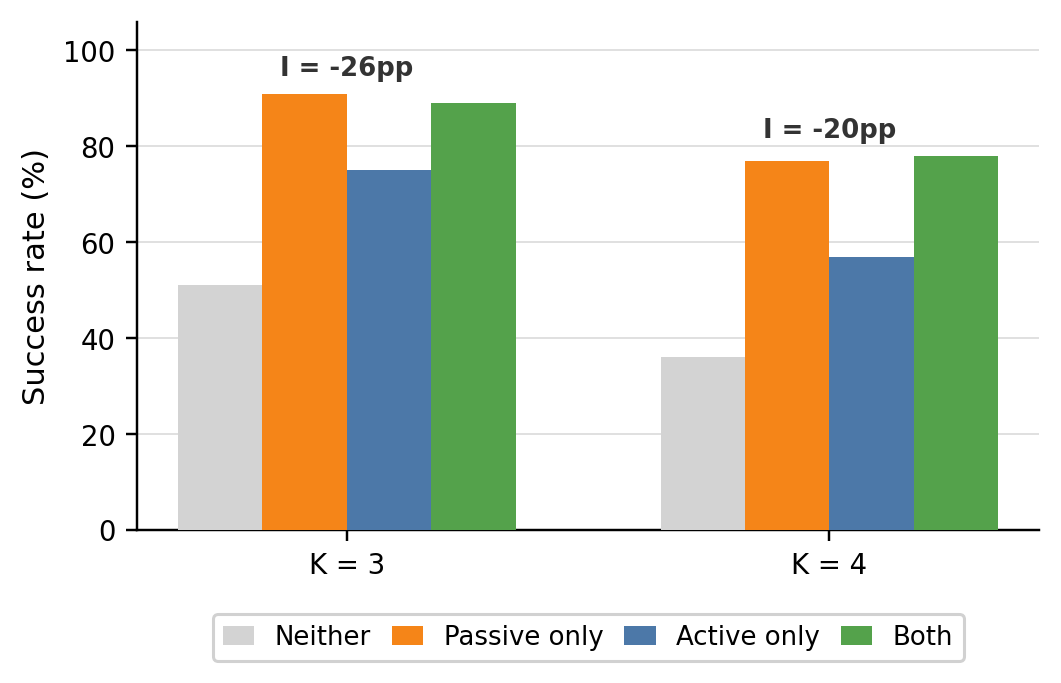
\includegraphics[width=\textwidth,height=3.8cm,keepaspectratio]{synergy_decomposition.png}\\[0.5em]
      \small\textbf{Watching and asking \alert{overlap}.}\\[0.2em]
      Their benefits don't add up ---\\
      asking matters most when watching fails.
    \column{0.48\textwidth}
      \centering
      
\includegraphics[width=\textwidth,height=3.8cm,keepaspectratio]{beta_inverted_u.png}\\[0.5em]
      \small\textbf{A \alert{more rational} partner\\ is \alert{not always easier} to help.}\\[0.2em]
      Their actions stop varying ---\\
      so a smart assistant asks \emph{more}.
  \end{columns}
\end{frame}

% =============================================================
\begin{frame}{When Watching Hurts --- and the Fix}
  \begin{columns}[T,onlytextwidth]
    \column{0.48\textwidth}
      \centering
      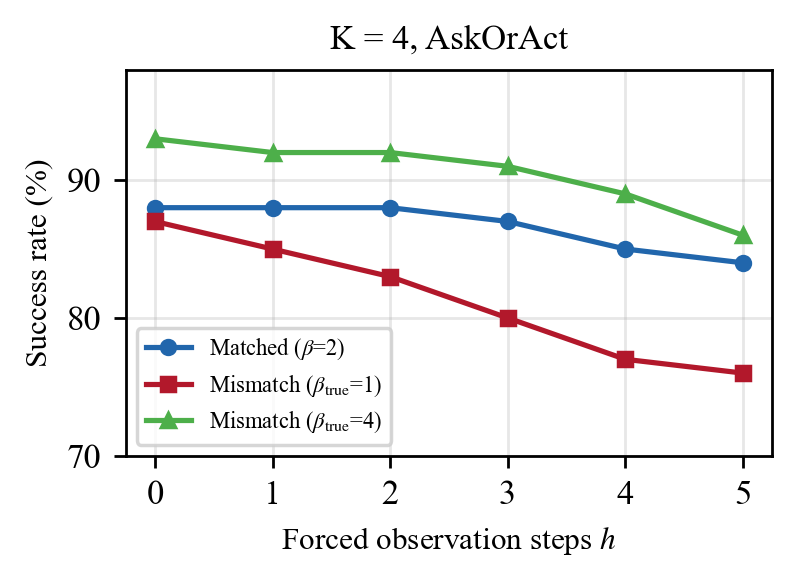
\includegraphics[width=\textwidth,height=3.8cm,keepaspectratio]{obs_hurts_mismatch.png}\\[0.4em]
      \small
      When the assistant's model is wrong,\\
      every extra step of watching\\
      makes things \alert{worse}, not better.
    \column{0.48\textwidth}
      \begin{block}{The fix}
        \small
        When an observation looks surprising,\\
        \textbf{trust it less.}\\[0.3em]
        Matched model: no harm.\\
        Wrong model: recovers the loss.
      \end{block}
      \vspace{0.5em}
      \begin{block}{Takeaways}
        \small
        \begin{enumerate}
          \item Watching and asking \emph{overlap} --- don't stack them.
          \item A more rational partner is not always easier.
          \item When your model is wrong, fix \emph{what you believe}, not \emph{when you speak}.
        \end{enumerate}
      \end{block}
  \end{columns}
\end{frame}

\appendix

% =============================================================
\begin{frame}{Appendix A: Prior Work Comparison}
  \footnotesize
  \centering
  \setlength{\tabcolsep}{4pt}
  \begin{tabular}{lcccccc}
    \toprule
    Feature & \rotatebox{60}{CLIPS} & \rotatebox{60}{GRD} & \rotatebox{60}{PAGR} & \rotatebox{60}{ATD} & \rotatebox{60}{ShootFirst} & \rotatebox{60}{\textbf{Ours}} \\
    \midrule
    Action-based goal inference & \checkmark & $\circ$ & \checkmark & -- & -- & \checkmark \\
    Explicit ask-or-act decision & -- & -- & $\circ$ & \checkmark & \checkmark & \checkmark \\
    Typed questions with cost $c_q$ & -- & -- & -- & \checkmark & -- & \checkmark \\
    Task completion, not just recognition & \checkmark & -- & -- & \checkmark & \checkmark & \checkmark \\
    Controlled ambiguity-$K$ sweep & -- & -- & -- & -- & -- & \checkmark \\
    Ground-truth task success & $\circ$ & -- & -- & -- & $\circ$ & \checkmark \\
    \bottomrule
  \end{tabular}

  \vspace{0.6em}
  \raggedright
  \scriptsize
  \checkmark\ present \quad $\circ$\ partial \quad -- absent
\end{frame}

\end{document}
